\documentclass[12pt, titlepage]{article}
\usepackage{listings}
\usepackage{hyperref}
\usepackage{amsmath, mathtools}
\usepackage{amsfonts}
\usepackage{amssymb}
\usepackage{graphicx}
\usepackage{colortbl}
\usepackage{xr}
\usepackage{longtable}
\usepackage{xfrac}
\usepackage{float}
\usepackage{siunitx}
\usepackage{caption}
\usepackage{pdflscape}
\usepackage{afterpage}
\usepackage{tabu}
\usepackage{verbatim}
\usepackage[round]{natbib}
\usepackage{url}
\usepackage{tikz}
\usepackage{enumitem}
\usepackage{extarrows}
\usepackage{booktabs}
\usepackage{tabularx}
\hypersetup{
    colorlinks,
    citecolor=black,
    filecolor=black,
    linkcolor=red,
    urlcolor=blue
}
\usepackage[round]{natbib}
\usepackage{fullpage}

%% Comments

\usepackage{color}

\newif\ifcomments\commentsfalse

\ifcomments
\newcommand{\authornote}[3]{\textcolor{#1}{[#3 ---#2]}}
\newcommand{\todo}[1]{\textcolor{red}{[TODO: #1]}}
\else
\newcommand{\authornote}[3]{}
\newcommand{\todo}[1]{}
\fi

\newcommand{\wss}[1]{\authornote{blue}{SS}{#1}}
\newcommand{\spc}[1]{\authornote{magenta}{SP}{#1}}
%% Common Parts

\newcommand{\progname}{MPS } % PUT YOUR PROGRAM NAME HERE

\externaldocument{../../SRS/SRS}

\newcounter{acnum}
\newcommand{\actheacnum}{AC\theacnum}
\newcommand{\acref}[1]{AC\ref{#1}}

\newcounter{ucnum}
\newcommand{\uctheucnum}{UC\theucnum}
\newcommand{\uref}[1]{UC\ref{#1}}

\newcounter{mnum}
\newcommand{\mthemnum}{M\themnum}
\newcommand{\mref}[1]{M\ref{#1}}

\newcounter{reqnum} %Requirement Number
\newcommand{\rthereqnum}{P\thereqnum}
\newcommand{\rref}[1]{R\ref{#1}}

\begin{document}

\title{CAS 741: Unit Verification and Validation Report\\[10pt]
\Large Dynamical Systems: \progname}
\author{Karol Serkis\\\texttt{serkiskj@mcmaster.ca}\\GitHub:
\href{https://www.github.com/karolserkis}{karolserkis}}
\date{\today}
	
\maketitle

\pagenumbering{roman}

\section{Revision History}

\begin{tabularx}{\textwidth}{p{3cm}p{2cm}X}
\toprule {\bf Date} & {\bf Version} & {\bf Notes}\\
\midrule
Dec. 18, 2018 & 1.0 &  First full draft for submission\\
\bottomrule
\end{tabularx}

~\newpage


\section{Symbols, Abbreviations and Acronyms}

See SRS Documentation at:\\
\url{https://github.com/karolserkis/CAS-741-Pendula/blob/master/docs/SRS/SRS.pdf}\\
The symbols are listed in alphabetical order.\\

\renewcommand{\arraystretch}{1.2}
\begin{tabular}{l l} 
  \toprule		
  \textbf{symbol} & \textbf{description}\\
  \midrule 
  A & Assumption\\
  DD & Data Definition\\
  FT & Functional Test \\
  GD & General Definition\\
  GS & Goal Statement\\
  IM & Instance Model\\
  LC & Likely Change\\
  MG & Module Guide\\ 
  MIS & Module Interface Specification\\ 
  NF & Non-Functional Requirement\\
  R & Requirement\\
  SRS & Software Requirements Specification\\
  T & Test\\
  VnV & Verification and Validation\\ 
  \bottomrule
\end{tabular}\\

\newpage

\tableofcontents

\listoftables %if appropriate

\listoffigures %if appropriate

\newpage


\pagenumbering{arabic}

This document is a review of the system tests that have been performed on 
\progname{}. This report is a partner to the Unit VnV Report that is located in 
the docs/VnVReport/UnitVnVReport directory.

\section{Functional Requirements Evaluation}

FR1 was: \progname program should be rendered with 3D Cartesian coordinates. \\
This requirement has been successfully met.\\

\noindent FR2 was: \progname program 
  will take the following inputs: 
  \begin{enumerate}
   \item The number of pendulum rods in the simulation. 
   \item Toggle the ground plane to introduce friction to the
   pendulum rod initial moment of inertia
   \item Toggle the plot of Potential \& Kinetic Energy
  \end{enumerate}
 This requirement has been successfully met.\\
                    
FR3 was: \progname program 
will calculate the kinetic and potential energy after the user has set the 
initialization parameters of input from the user have been entered.\\
This requirement has been successfully met.\\

FR4 was: \progname program 
will calculate the Lagrangian after the user has set the initialization 
parameters of input have been entered and the kinetic and potential energy of 
the system as whole has been calculated.
This requirement has been somewhat met. A generic use of OpenGL and GLUT
has allowed for other ways around this.\\

FR5 was: \progname program
will ensure that the inputs do not violate the constraints specified in the 
Data Constraints section:
    \begin{enumerate} \item \progname program will 
generate diagrams with and plot lines and time-line of logged movement. 
\item The time-line of swings of the pendulum will be logged and eventually
return to a resting state in equilibrium
\end{enumerate} 
This requirement has been somewhat successfully met.\\

\section{Nonfunctional Requirements Evaluation}

NFR1 and subsequent requirements for the software to be portable have been met.\\
The simulation software can run on any computer system and is contained in one 
Python file for convenience.

\subsection{Usability}

To make the program easy to use, the interaction with the GUI is minimal. \\
The user can provide a variety of input types, but because of exception handling
the program will still run or provide feedback to let the user try the correct input 
parameters into the command-line.
		
\subsection{Performance}

The performance bottleneck is most likely the running of the program 
on a local computer. The simulation requires some relative graphics card for 
calculations. Performance otherwise is not a focus of the program.
	
\section{Comparison to Existing Implementation}	

Comparing Existing Implementation resulted in very comparable results
thus the simulation was quite capable and true to life.

\section{Unit Testing}

The unit testing will be covered in more details in the UnitVnVReport. The 
actual implementation of the unit tests can be found in the src/ or test/ 
directory on the github repo \url{https://github.com/karolserkis/CAS-741-Pendula}.

\section{Changes Due to Testing}

The actual Unit VnV Plan tests will be discussed henceforth. All 
the functional and most of the non-functional requirements have been meet.

\section{Automated Testing}

Unit-based scripts can be created for testing the modules in \progname{}and be tested automatically with 
scripts written in pytest. The test scripts using pytest will cycle through an array of data and check an assert 
statement. See section on verification tools for more information.

\begin{figure}[H]
	\centering
	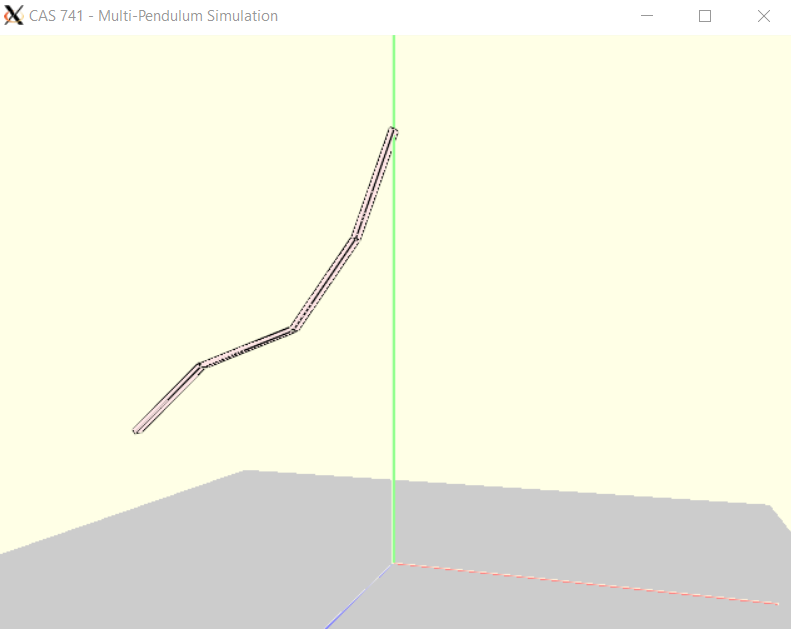
\includegraphics[width=400px]{MPSim.PNG}
	\caption{Kinetic and potential energy and simulation
	of multi-rod pendulum chain~\citep{WikipediaPendulum}}
	\label{fig:PE-pend}
\end{figure}
		
\section{Trace to Requirements}

All functional requirements met.
\begin{table}[H]
	\centering
	\begin{tabular}{p{0.2\textwidth} p{0.6\textwidth}}
		\toprule
		\textbf{Req.} & \textbf{Modules}\\
		\midrule
		R1 & MPSim.py  \\
		R2 & MPSim.py  \\
		R3 & MPSim.py  \\
		R4 & MPSim.py  \\
		R5 & MPSim.py, MPSim\_inputargparse\_test.py \\
		NFR1 & MPSim.py \\
		\bottomrule
	\end{tabular}
	\caption{Trace between requirements and modules, with the specific python 
	file names given (as found in the kaplan directory). A similar table is 
	found in the module guide document.}
	\label{trace-RM}
\end{table}	
		
\section{Trace to Modules}		

\begin{table}[H]
\begin{center}

	\centering
	\begin{tabular}{p{0.3\textwidth} p{0.45\textwidth} p{0.3\textwidth}}
		\toprule
		\textbf{Module} & \textbf{Test File} & \textbf{Comments} \\
		\midrule
		M1 (Hardware Hiding) & - & Out of scope \\
		M2 (MPSim Control) & MPSim.py, MPSim\_inputargparse\_test.py  & complete \\
		M3 (Generic GUIl) & MPSim.py, MPSim\_inputargparse\_test.py  & complete \\
		M3 (User Input) & MPSim.py, MPSim\_inputargparse\_test.py  & complete \\
		M5 (Lagrangian Module) & MPSim.py, MPSim\_inputargparse\_test.py  & complete \\
		M6 (Data Structure) & MPSim.py & incomplete \\
		M7 (Generic Plot) & MPSim.py & complete for current spec \\
		M8 (Generic Trajectory) & MPSim.py & complete for current spec \\
		\bottomrule
	\end{tabular}
	\caption{Trace between modules and tests, with the specific python 
		file names given (as found in the kaplan/test directory), or (if no 
		python test was written) a comment or reference to a jupyter notebook 
		(located in the kaplan/test/jupyter-notebooks directory).}
	\label{trace-MT}

\end{center}
\end{table}	

\section{Code Coverage Metrics}

Current code coverage metrics can be found in the test scripts 
using pytest will cycle through an array of data and check an assert 
statement. See section on verification tools for more information.
\begin{lstlisting}[language=python, showstringspaces=false]

Name                                         Cover
----------------------------------------------------------------
src/MPSim.py                                1/3 tests
src/MPSim_inputargparse_test.py             7/8 tests
test/sim_inputargparse_test.py              7/8 tests
---------------------------------------------------------------
$ pytest-3
============= test session starts==================================
platform linux -- Python 3.6.7, pytest-3.3.2, py-1.5.2, pluggy-0.6.0
rootdir: /mnt/c/Users/Karol/CAS-741-Pendula/src, inifile:
collected 8 items

MPSim_inputargparse_test.py .......x                                                                                                                               [100%]

============ 7 passed, 1 xfailed in 2.19 seconds ==================
\end{lstlisting}

\bibliographystyle{plainnat}

\bibliography{../../../ReferenceMaterial/References}

\end{document}
